\documentclass[11pt]{article}
\usepackage[top=1in, bottom=1.25in, left=1.25in, right=1.25in]{geometry}
\newcommand{\tabitem}{~~\llap{\textbullet}~~}
\usepackage[parfill]{parskip}
\usepackage{enumerate,amsmath,amsthm,amssymb,bbold}
\usepackage{minibox,graphicx,caption,booktabs,pdflscape,multirow,verbatim,subcaption,pdfpages,longtable}
\usepackage[shortlabels]{enumitem}
\usepackage[T1]{fontenc}
\usepackage[section]{placeins} %to keep graphs and tables in the very section to which they belong 
\usepackage{adjustbox}
%-----------------------------------------------------------------------------
\begin{document}
\begin{center}
\framebox[\linewidth]{ 
	\minibox[c]{
	\Large Homework \#3 \\ \\
	Professor: Pat Kline \\ \\
	Students: Christina Brown, Sam Leone, Peter McCrory, Preston Mui
	}
}
\end{center}

\bigskip \textbf{Reweighting}

\bigskip \textit{Subproblem A}

\bigskip First, the authors drop a number of demographic groups from their analysis: those self-employed, those under 18 or over 64, and those with more than 38 years of work experience.\footnote{The authors merely \textit{note} these data-build decisions in their cleaning .do files, they do not \textit{implement} them there.} To compare these groups to prime-working-age employees would be to compare apples and oranges. Second, they top code the wage. This prevents outliers from skewing the analysis. Third, they round school years to whole numbers. This makes the analysis easier in terms of both implementation and interpretation.\footnote{We thank Isabelle Cohen for helpful discussions on this subproblem.}

\bigskip \textit{Subproblem B}

\begin{figure}[H]
	\caption{Kernel Density for Full Sample}
	\centering
	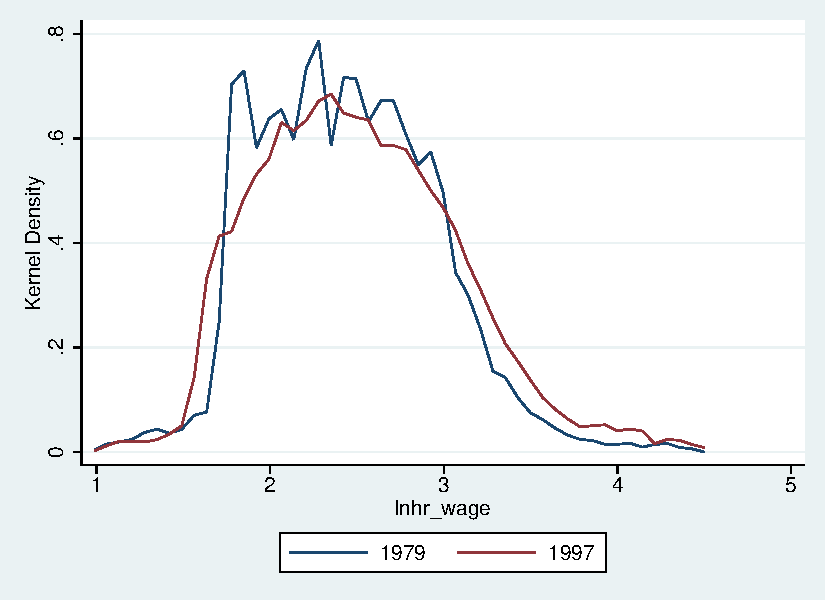
\includegraphics[width=.75\textwidth]{Kernel_Density_Full.pdf}
\end{figure}

\textit{Subproblem C}

\bigskip The 1997 wage distribution has more mass at the tails than does the 1979 wage distribution. This is in keeping with the authors' result that wage inequality has increased over the past two decades. The 1997 wage distribution also appears to be skewed right. This is in keeping with the authors' result that increasing wage inequality is driven more by the 90/50 gap than by 50/10 gap.

\bigskip In addition, there appears to be bunching at the low-end of the 1979 distribution. This is in keeping with the hypothesis - which the authors comment on but do not argue for - that the minimum wage has been an important determinant of the U.S. wage distribution over the past decades.

\bigskip The key now is to disentangle the degree to which these changes come from (a) the changing demographic composition of the labor force (what you might call ``selection") and (b) more fundamental labor-market changes happening within demographic groups (what you might call ``treatment"). Read on!

\bigskip \textit{Subproblem D}

\begin{figure}[H]
	\caption{Kernel Density for Selected Subsamples}
	\begin{subfigure}[H]{.5\textwidth}
		\caption{Kernel Density for Black Men Aged 25-50}
		\centering
		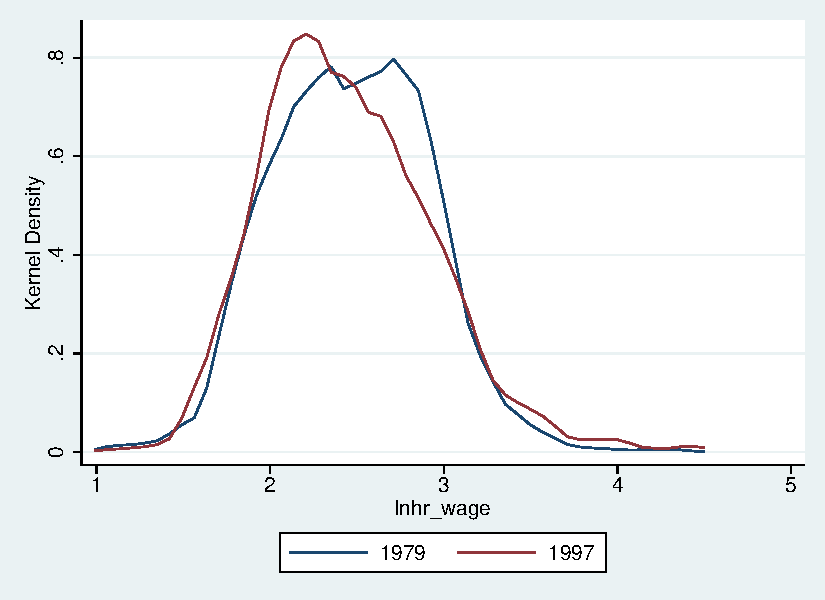
\includegraphics[width=1\textwidth]{Kernel_Density_Black_Men.pdf}
	\end{subfigure}
	\hfill
	\begin{subfigure}[H]{.5\textwidth}
		\caption{Kernel Density for White Women Aged 25-50}
		\centering
		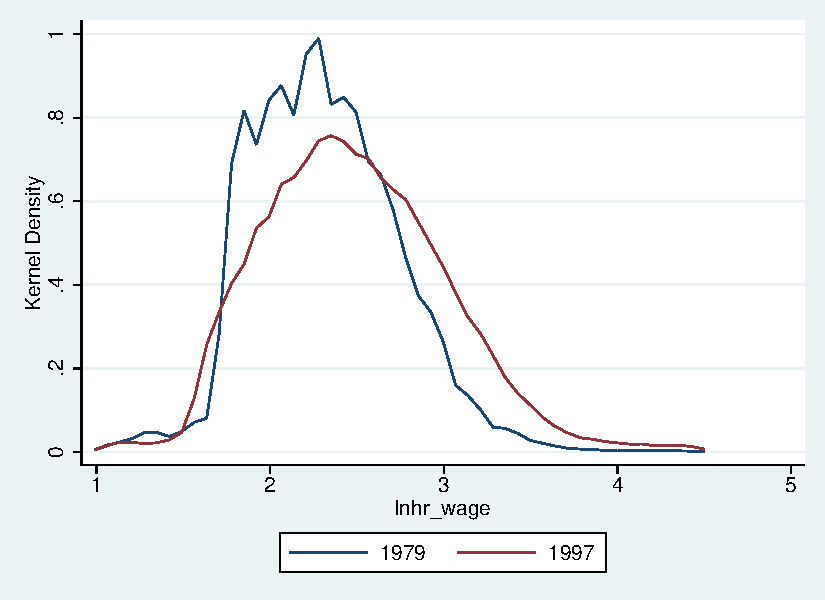
\includegraphics[width=1\textwidth]{Kernel_Density_White_Women.pdf}
	\end{subfigure}
\end{figure}

There were more women and minorities (e.g. black and Latinos) in the labor force in 1997 than in 1979. Could this demographic shift alone explain the changes in the overall wage distribution? Probably not: When we plot the wage distributions specifically for young black men and young black women, we still changes between 1979 and 1997. In other words, even conditioning on these particular demographic characteristics, we still see that there are more fundamental economic forces at work.

\bigskip So: What changes do we see exactly? For black men, the mean wage is actually lower in 1997 than it was in 1979. This could be because of increased racial discrimination, changes in government welfare programs, or changes in the skill level of the average African-American worker (e.g. if a higher portion of African Americans were working in 1997 than in 1979, the average worker might be less skilled). For white women, the mean wage is higher in 1997 than it was in 1979, and overall the distribution is more symmetric. This is unsurprising, since women were more likely to hold high-skill/high-wage positions in the late 1990s than in the late 1970s.

\bigskip Compared to the overall distribution, white woman have a similar average wage, but black men have a lower average wage.

\bigskip \textit{Subproblem E}

\bigskip See the attached Stata code.

\bigskip \textit{Subproblems F \& G}

\begin{figure}[H]
	\caption{Actual 1997 vs. Counterfactual 1997}
	\centering
	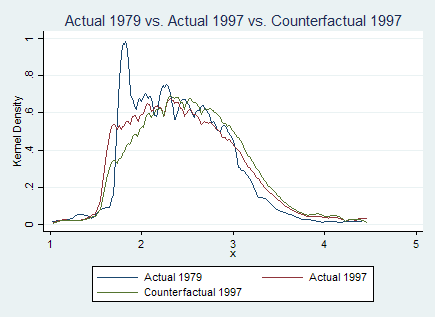
\includegraphics[width=.75\textwidth]{Kernel_Density_1997_C1997.png}
\end{figure}

\begin{figure}[H]
	\caption{Actual 1979 vs. Counterfactual 1979}
	\centering
	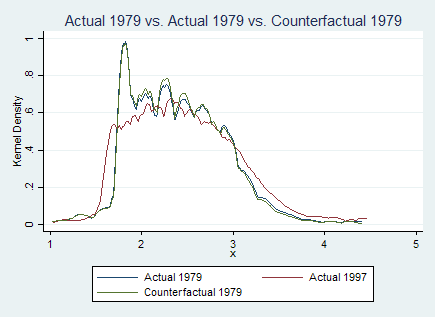
\includegraphics[width=.75\textwidth]{Kernel_Density_1979_C1979.png}
\end{figure}

%\begin{figure}[H]
%	\caption{What the fuck do these graphs tell us?}
%	\begin{subfigure}[H]{.5\textwidth}
%		\caption{Actual 1997 vs. Counterfactual 1979}
%		\centering
%		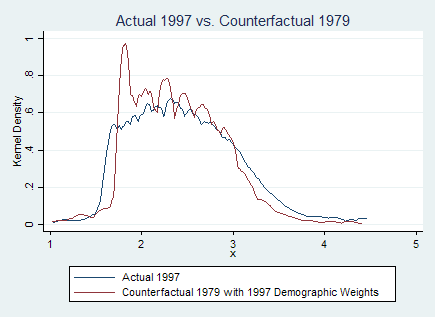
\includegraphics[width=1\textwidth]{Kernel_Density_1997_C1979.png}
%	\end{subfigure}
%	\hfill
%	\begin{subfigure}[H]{.5\textwidth}
%		\caption{Actual 1979 vs. Counterfactual 1997}
%		\centering
%		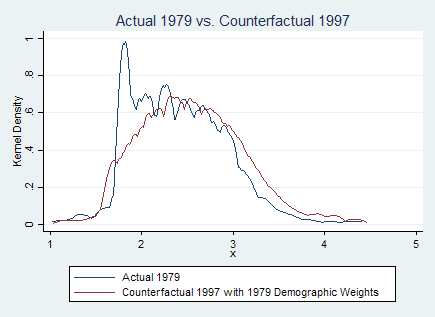
\includegraphics[width=1\textwidth]{Kernel_Density_1979_C1997.png}
%	\end{subfigure}
%\end{figure}

\textit{Subproblem H}

\bigskip Above, when we estimated separate wage distributions for young black men and young white women, we were going some of the way toward disentangling demographic effects from more fundamental economic effects. But we can still go further. One strategy is to \textit{reweight} the 1997 sample so that it has the same demographic shares as the 1997 sample. We would then have a new \textit{counterfactual} 1997 wage distribution. And we we moved from one distribution to another, we would then be able to isolate one of our effects of interest:

$$ \text{Actual 1979} \underbrace{\Rightarrow}_{Fundamentals} \text{Reweighted 1997} \underbrace{\Rightarrow}_{Demographics} \text{Actual 1997} $$

\bigskip How can we produce the weights exactly?\footnote{We thank Christopher Campos for help with this mathematical explication.} Let $w$ be the wage schedule, let $z$ be demographic characteristics, and let $t$ be the year. Let the conditional pdf of $w$ be $f(w|t_w=t,t_z=t)$. Notice that $t$ is indexed by $w$ and by $z$, which indicates that we can, counterfactually, mix wage schedules and demographic characteristics from different years. For example, conditioning $t_w=1979,t_z=1997$ means conditioning on the wage schedule that prevailed in 1979 but the demographic characteristics that prevailed in 1997.

%With this notation, the pdf of wages is as follows.
%\begin{align*}
%f_t(w) &= \int_{z} dF(w,z|t_{w,z}=t) \\
%&= \int_{z} f(w|z,t_{w,z}=t)dF(z|t_z=t) \\
%&= f(w|t_w=t,t_z=t)
%\end{align*}

\bigskip Consider the baseline case, where we reweight the 1997 wage distribution so that it has the 1979 demographic characteristics.

\begin{align*}
f(w|t_w=1997,t_z=1979)&=\int_{z} f(w|z,t_w=1997)dF(z|t_z=1979) \\
&=\int_{z} f(w|z,t_w=1997)\frac{dF(z|t_z=1997)}{dF(z|t_z=1997)}dF(z|t_z=1979) \\
&=\int_{z} f(w|z,t_w=1997)\Psi_z(z)dF(z|t_z=1997)
\end{align*}

where

$$ \Psi_z(z) = \frac{dF(z|t_z=1979)}{dF(z|t_z=1997)} $$

By Bayes' Rule

\begin{align*}
\Psi_z(z) &=\frac{dF(z|t_z=1979)}{dF(z|t_z=1997)} \\
&=\frac{P(t_z=1979|z)F(z)}{P(t_z=1979)}\frac{P(t_z=1997)}{P(t_z=1997|z)F(z)} \\
&= \frac{P(t_z=1979|z)}{P(t_z=1997|z)}\frac{P(t_z=1997)}{P(t_z=1979)}
\end{align*}

where the conditional probabilities are are the sample frequencies and the unconditional probabilities are propensity scores.

\bigskip In this case, $\Psi_z(z)dF(z|t_z=1997)$ yields the new weights. Boom! (See the attached Stata code for the actual logistic regression specification used to produce the propensity scores.)

\bigskip Figure 3 plots the three distributions on top of each other. We can apply this logic to our problem at hand: Observe Figure 3 above. Start with the actual 1979 distribution (blue line) and move to the reweighted 1997 distribution (green line). There is a big change. Now move to the actual 1997 distribution (red line). There is a small change. This suggests that the evolution of the wage distribution is not merely due to demographic characteristics, but rather results from other economic forces affecting the wage schedule.

\bigskip The same logic applies going backward in time instead of forward in time. Observe Figure 4, which instead plots the counterfactual 1979 distribution using 1997 weights. There is a big difference between the actual 1997 distribution (red line) and the reweighted 1979 distribution (green line), but not between the reweighted 1979 distribution and the actual 1979 distribution (blue line). This serves as a robustness check, and provides further evidence that more fundamental economic forces are at play.

\bigskip \textit{Subproblem I}

\begin{table}[H]\centering
	\caption{Actual 1979}{\label{} 
		\textbf{} }\begin{tabular} {@{} l r r r r r r r @{}} \\ \hline
		\textbf{variable } & \textbf{      mean} & \textbf{        sd} & \textbf{       p10} &
		\textbf{       p25} & \textbf{       p50} & \textbf{       p75} & \textbf{       p90} \\
		\hline
		age  &   34.99355 &   12.77136 &         20 &         24 &         32 &        
		45 &         55 \\
		\hline
		%\multicolumn{8}{@{}l}{\footnotesize{\emph{Source:} ./morg_cleaned_1980-occ.dta}}
	\end{tabular}
\end{table}

\begin{table}[H]\centering
	\caption{Counterfactual 1997 Reweighted with 1979 Demographic Characteristics}{\label{} 
		\textbf{} }\begin{tabular} {@{} l r r r r r r r @{}} \\ \hline
		\textbf{variable } & \textbf{      mean} & \textbf{        sd} & \textbf{       p10} &
		\textbf{       p25} & \textbf{       p50} & \textbf{       p75} & \textbf{       p90} \\
		\hline
		age  &   38.94351 &   9.939499 &         26 &         32 &         39 &        
		46 &         52 \\
		\hline
		%\multicolumn{8}{@{}l}{\footnotesize{\emph{Source:} ./morg_cleaned_1980-occ.dta}}
	\end{tabular}
\end{table}

\bigskip \textit{Subproblem J}

\begin{table}[H]\centering
	\caption{Actual 1979 (African Americans)}{\label{} 
		\textbf{} }\begin{tabular} {@{} l r r r r r r r @{}} \\ \hline
		\textbf{variable } & \textbf{      mean} & \textbf{        sd} & \textbf{       p10} &
		\textbf{       p25} & \textbf{       p50} & \textbf{       p75} & \textbf{       p90} \\
		\hline
		age  &   35.52812 &   12.33177 &         21 &         25 &         33 &        
		45 &         54 \\
		\hline
		%\multicolumn{8}{@{}l}{\footnotesize{\emph{Source:} ./morg_cleaned_1980-occ.dta}}
	\end{tabular}
\end{table}

\begin{table}[H]\centering
	\caption{Counterfactual 1997 Reweighted with 1979 Demographic Characteristics (African Americans)}{\label{} 
		\textbf{} }\begin{tabular} {@{} l r r r r r r r @{}} \\ \hline
		\textbf{variable } & \textbf{      mean} & \textbf{        sd} & \textbf{       p10} &
		\textbf{       p25} & \textbf{       p50} & \textbf{       p75} & \textbf{       p90} \\
		\hline
		age  &   38.19553 &   9.680713 &         25 &         31 &         38 &        
		45 &         51 \\
		\hline
		%\multicolumn{8}{@{}l}{\footnotesize{\emph{Source:} ./morg_cleaned_1980-occ.dta}}
	\end{tabular}
\end{table}

\bigskip \textit{Subproblem K \& L}

\bigskip Observe from Tables 1-4 that, at least for age, the 1979 and the reweighted 1997 distributions do not have the same moments/quantiles. This is problematic, since the weights are supposed to have been calculated in order to achieve similar demographic characteristics between the two distributions. This suggests that our propensity scores might be misspecified. Below we try a few different specifications, namely (a) adding a cubic term in age, and (b) eliminating the quadratic term in age. Neither makes a difference.

\begin{table}[H]\centering
	\caption{Actual 1979: Logit with Age, Age$^2$, Age$^3$}{\label{} 
		\textbf{} }\begin{tabular} {@{} l r r r r r r r @{}} \\ \hline
		\textbf{variable } & \textbf{      mean} & \textbf{        sd} & \textbf{       p10} &
		\textbf{       p25} & \textbf{       p50} & \textbf{       p75} & \textbf{       p90} \\
		\hline
		age  &   34.99355 &   12.77136 &         20 &         24 &         32 &        
		45 &         55 \\
		\hline
		%\multicolumn{8}{@{}l}{\footnotesize{\emph{Source:} ./morg_cleaned_1980-occ.dta}}
	\end{tabular}
\end{table}

\begin{table}[H]\centering
	\caption{Counterfactual 1997: Logit with Age, Age$^2$, Age$^3$}{\label{} 
		\textbf{} }\begin{tabular} {@{} l r r r r r r r @{}} \\ \hline
		\textbf{variable } & \textbf{      mean} & \textbf{        sd} & \textbf{       p10} &
		\textbf{       p25} & \textbf{       p50} & \textbf{       p75} & \textbf{       p90} \\
		\hline
		age  &   39.18865 &   9.905478 &         26 &         32 &         39 &        
		46 &         52 \\
		\hline
		%\multicolumn{8}{@{}l}{\footnotesize{\emph{Source:} ./morg_cleaned_1980-occ.dta}}
	\end{tabular}
\end{table}

\begin{table}[H]\centering
	\caption{Actual 1979: Logit with Age, Age$^2$, Age$^3$ (African Americans)}{\label{} 
		\textbf{} }\begin{tabular} {@{} l r r r r r r r @{}} \\ \hline
		\textbf{variable } & \textbf{      mean} & \textbf{        sd} & \textbf{       p10} &
		\textbf{       p25} & \textbf{       p50} & \textbf{       p75} & \textbf{       p90} \\
		\hline
		age  &   35.52812 &   12.33177 &         21 &         25 &         33 &        
		45 &         54 \\
		\hline
		%\multicolumn{8}{@{}l}{\footnotesize{\emph{Source:} ./morg_cleaned_1980-occ.dta}}
	\end{tabular}
\end{table}

\begin{table}[H]\centering
	\caption{Counterfactual 1997: Logit with Age, Age$^2$, Age$^3$ (African Americans)}{\label{} 
		\textbf{} }\begin{tabular} {@{} l r r r r r r r @{}} \\ \hline
		\textbf{variable } & \textbf{      mean} & \textbf{        sd} & \textbf{       p10} &
		\textbf{       p25} & \textbf{       p50} & \textbf{       p75} & \textbf{       p90} \\
		\hline
		age  &   38.46548 &   9.677537 &         25 &         31 &         38 &        
		46 &         51 \\
		\hline
		%\multicolumn{8}{@{}l}{\footnotesize{\emph{Source:} ./morg_cleaned_1980-occ.dta}}
	\end{tabular}
\end{table}

\begin{table}[H]\centering
	\caption{Actual 1979: Logit with Age Only}{\label{} 
		\textbf{} }\begin{tabular} {@{} l r r r r r r r @{}} \\ \hline
		\textbf{variable } & \textbf{      mean} & \textbf{        sd} & \textbf{       p10} &
		\textbf{       p25} & \textbf{       p50} & \textbf{       p75} & \textbf{       p90} \\
		\hline
		age  &   34.99355 &   12.77136 &         20 &         24 &         32 &        
		45 &         55 \\
		\hline
		%\multicolumn{8}{@{}l}{\footnotesize{\emph{Source:} ./morg_cleaned_1980-occ.dta}}
	\end{tabular}
\end{table}

\begin{table}[H]\centering
	\caption{Counterfactual 1997: Logit with Age Only}{\label{} 
		\textbf{} }\begin{tabular} {@{} l r r r r r r r @{}} \\ \hline
		\textbf{variable } & \textbf{      mean} & \textbf{        sd} & \textbf{       p10} & \textbf{       p25} & \textbf{       p50} & \textbf{       p75} & \textbf{       p90} \\
		\hline
		age  &   39.35282 &   11.33751 &         24 &         31 &         39 &         48 &         55 \\
		\hline
		%\multicolumn{8}{@{}l}{\footnotesize{\emph{Source:} ./morg_cleaned_1980-occ.dta}}
	\end{tabular}
\end{table}


\begin{table}[H]\centering
	\caption{Actual 1979: Logit with Age Only (African Americans)}{\label{} 
		\textbf{} }\begin{tabular} {@{} l r r r r r r r @{}} \\ \hline
		\textbf{variable } & \textbf{      mean} & \textbf{        sd} & \textbf{       p10} &
		\textbf{       p25} & \textbf{       p50} & \textbf{       p75} & \textbf{       p90} \\
		\hline
		age  &   35.52812 &   12.33177 &         21 &         25 &         33 &        
		45 &         54 \\
		\hline
		%\multicolumn{8}{@{}l}{\footnotesize{\emph{Source:} ./morg_cleaned_1980-occ.dta}}
	\end{tabular}
\end{table}

\begin{table}[H]\centering
	\caption{Counterfactual 1997: Logit with Age Only (African Americans)}{\label{} 
		\textbf{} }\begin{tabular} {@{} l r r r r r r r @{}} \\ \hline
		\textbf{variable } & \textbf{      mean} & \textbf{        sd} & \textbf{       p10} &
		\textbf{       p25} & \textbf{       p50} & \textbf{       p75} & \textbf{       p90} \\
		\hline
		age  &   38.41906 &   11.01582 &         24 &         30 &         38 &        
		47 &         54 \\
		\hline
		%\multicolumn{8}{@{}l}{\footnotesize{\emph{Source:} ./morg_cleaned_1980-occ.dta}}
	\end{tabular}
\end{table}

\bigskip \textbf{Matching}

\begin{enumerate}[(a)]

	\item To run OLS on $Y_{i2} - Y_{i1} = \gamma_2 - \gamma_1 + \beta D_{i2} + \epsilon_{i2} - \epsilon_{i1}$, the identifying restriction is that $E\left[D_{i2} (\epsilon_{i2} - \epsilon_{i1})\right] = 0$; that is, program participation is uncorrelated with the change in error terms $\epsilon_{i2} - \epsilon_{i1}$.

	\item $Y_{i2} = Y_{i1} + (\gamma_2 - \gamma_1) + \beta D_{i2} + \epsilon_{i2} - \epsilon_{i1}$

	\item Taking expectations,
	\begin{align*}
		E\left[Y_{i2} | Y_{i1}, D_{i2} = 1\right] &= Y_{i1} + (\gamma_2 - \gamma_1) + \beta + E[\epsilon_{i2} - \epsilon_{i1} | Y_{i1}, D_{i1}=1]\\
		E\left[Y_{i2} | Y_{i1}, D_{i2} = 0\right] &= Y_{i1} + (\gamma_2 - \gamma_1) + E[\epsilon_{i2} - \epsilon_{i1} | Y_{i1}, D_{i1}=0]
	\end{align*}
	the difference of these two identifies $\beta$ if
	\begin{align*}
		E[\epsilon_{i2} - \epsilon_{i1} | Y_{i1}, D_{i2}=1] - E[\epsilon_{i2} - \epsilon_{i1} | Y_{i1}, D_{i2}=0] &= 0 \\
		E \bigg[ E[\epsilon_{i2} - \epsilon_{i1} | D_{i2}=1] - E[\epsilon_{i2} - \epsilon_{i1} | D_{i2}=0] \bigg| Y_{i1} \bigg]&= 0 \\
		E \bigg[ D_{i2} (\epsilon_{i2} - \epsilon_{i1}) \bigg| Y_{i1} \bigg]&= 0 \\
	\end{align*}
	
	\item This assumption is stricter than that of the assumption in part (a); it is the same restriction in part (a), but conditional on $Y_{i1}$.

	\item The Smith and Todd (2005) matched differences-in-differences estimator requires that selection is independent on the differences in untreated outcomes between time periods, conditional on the propensity. Formally,
	\begin{align*}
		E \bigg[ D_{i2} (\gamma_2 + \epsilon_{i2} - \gamma_1 - \epsilon_{i1} ) \bigg| P_{i} \bigg] &= E[D_{i2}] E \bigg[  (\gamma_2 + \epsilon_{i2} - \gamma_1 - \epsilon_{i1} ) \bigg| P_{i} \bigg] \\
		\implies E \bigg[ D_{i2} (\epsilon_{i2} - \epsilon_{i1} ) \bigg| P_{i} \bigg] &= 0
	\end{align*}
	which is the same condition from above, except instead of conditioning on $Y_{i1}$ we are conditioning on $P_i$, the conditions are not really ``weaker'' than the ones above.

\end{enumerate}


\bigskip \textbf{2SLS}

\begin{enumerate}[(a)]

	\item The moment conditions defining the 2SLS estimator are
	\begin{align*}
		E \left[ Z_i \epsilon_i \right] &= 0 \\
		E \left[ Z_i^2 \epsilon_i \right] &= 0
	\end{align*}
	they imply each other, since functions of uncorrelated variables are uncorrelated with each other.

	\item The moment conditions defining the control function estimator are
	\begin{align*}
		E \left[ Z_i \epsilon_i \right] &= 0 \\
		E \left[ Z_i v_i \right] &= 0 \\
		E \left[ \epsilon_i | v_i \right] &= \rho \frac{\sigma_{\epsilon}}{\sigma_v} v_i \\
		E \left[ (Y_i - \beta_0 - \beta_1 X_i - \beta_2 X_i^2 - \rho \frac{\sigma_{\epsilon}}{\sigma_v} v_i)X_i \right] &= 0 \\
		E \left[ (Y_i - \beta_0 - \beta_1 X_i - \beta_2 X_i^2 - \rho \frac{\sigma_{\epsilon}}{\sigma_v} v_i)X_i^2 \right] &= 0 \\
		E \left[ (Y_i - \beta_0 - \beta_1 X_i - \beta_2 X_i^2 - \rho \frac{\sigma_{\epsilon}}{\sigma_v} v_i)v_i \right] &= 0
	\end{align*}

	\item The control function estimator relies on stronger conditions than the 2SLS estimator. The only condition in the 2SLS estimator is that the instrument, $Z$, is uncorrelated with the error term $\epsilon$. However, the control function estimator relies on specifying the exogenous relationship between $X$ and $Z$, in particular that the conditional expection of $X$ given $Z$ is linear.

	\item The control function would work better when $Z$ is weak, because it brings to bear more moment restrictions than the 2SLS estimator, whereas the 2SLS estimator only relies on the exogeneity of $Z$. %Should add more but not sure what

	\item

	The table below contains the estimates for $\beta_1$ and $\beta_2$ under the 2SLS and control function methods.

	\begin{enumerate}[(i)]
	 
		\item Overall, for all values of $\gamma$, the control function estimate appears to be more efficient (the spread of the estimates is much lower), because the control function's ``first-stage'' is correctly specified, and the estimation involves more moment restrictions.
		
		\item As $\gamma_1$ shrinks, the mean 2sls estimate falls (away from the true value of $1.0$), although the median appears to remain unbiased. The interquartile range of both estimators increases, although the IQR for the 2sls estimate increases much faster than that of the control function. The control function estimates appear to remain both median and mean-unbiased.

		\item If one wanted to test the hypothesis that $\rho \frac{\sigma_{\epsilon}}{\sigma_{v}} = 0$, one would need an additional term in the variance of the coefficient on $v_i$. In particular, by using the two-stage estimate formulas for the asymptotic variance of the estimate of $\rho \frac{\sigma_{\epsilon}}{\sigma_{v}}$, one would see that in the ``sandwich'' estimator, one would replace the term
		\begin{align*}
			E[s_i(\theta_0, \gamma^*)s_i(\theta_0, \gamma^*)']
		\end{align*}
		where $\theta_0 = (\beta_0, \beta_1, \beta_2, \rho \frac{\sigma_{\epsilon}}{\sigma_{v}})$ and $\gamma^* = (\gamma_0, \gamma_1)$, and $s_i$ being the score function (gradient of the squared residual with respect to $\theta_0$), with this term
		\begin{align*}
			& E[g_i(\theta_0, \gamma^*)g_i(\theta_0, \gamma^*)'] \\
			\mbox{s. t. } g_i(\theta_0, \gamma^*) &\equiv s_i(\theta_0, \gamma^*) + E \left[ \nabla_\gamma s_i(\theta_0, \gamma^*) \right]  r_i (\theta_0, \gamma^*)
		\end{align*}
		where $r_i$ is the asymptotic variance of $\sqrt{N}(\hat{\gamma} - \gamma^*)$ and can be obtained from the ``first-stage'' regression. To construct an estimate of the standard error, one can simply plug in the population analogues into this sandwich estimator and run a t-test with the modified standard error.

	\end{enumerate}

	\centering
	
\begin{tabular}{|l|c|c|c|c|}
\hline
Statistic & $\beta_1^{2sls}$ & $\beta_2^{2sls}$ & $\beta_1^{cf}$ & $\beta_2^{cf}$ \\ \hline
\multicolumn{5}{|c|}{$\gamma = 0.3$} \\ \hline
mean & 1.003234 & 1.076318 & .9938653 & 1.000297 \\
sd & .3412886 & 3.060352 & .1081107 & .0204986 \\
p50 & .9992083 & .9904965 & .9961268 & 1.000156 \\
iqr & .1585197 & .3704991 & .1449331 & .0277689 \\ \hline
\multicolumn{5}{|c|}{$\gamma = 0.2$} \\ \hline
mean & .7418318 & 2.253272 & .9936412 & .999546 \\
sd & 8.550667 & 47.84852 & .1688314 & .0207697 \\
p50 & .9829823 & 1.005342 & .9991214 & .9994298 \\
iqr & .315193 & .7726767 & .2297587 & .0277564 \\ \hline
\multicolumn{5}{|c|}{$\gamma = 0.1$} \\ \hline
mean & .8100506 & .839673 & .9693889 & .9988507 \\
sd & 7.576605 & 17.05286 & .5007757 & .0224328 \\
p50 & 1.029302 & 1.044092 & 1.005126 & .9992241 \\
iqr & .7045021 & 1.448808 & .4600121 & .0299107 \\ \hline
\end{tabular}

% ->  gamma = .2
% \begin{tabular}
% Statistic & $\beta_1^{2sls}$ & $\beta_2^{2sls}$ & $beta_1^{cf}$ & $beta_2^{cf}$ \\ \hline
% mean & .7418318 & 2.253272 & .9936412 & .999546 \\
% sd & 8.550667 & 47.84852 & .1688314 & .0207697 \\
% p50 & .9829823 & 1.005342 & .9991214 & .9994298 \\
% iqr & .315193 & .7726767 & .2297587 & .0277564 \\ \hline
% \end{tabular}

% \begin{tabular}
%   Statistic & $\beta_1^{2sls}$ & $\beta_2^{2sls}$ & $beta_1^{cf}$ & $beta_2^{cf}$ \\ \hline

% \end{tabular}


\end{enumerate}

\bigskip \textbf{Bootstrap OLS}

\begin{enumerate}[(a)]
	\item See the regression results in table below. The clustered standard error on D is 0.0925.
	\item The p value for the null hypothesis that the coefficient on D equals zero is 0.008.
	\item See column 2 of the table below. Using a block bootstrap our new standard error on D is 0.0965 and the p value is 0.003.
	\item The p value of the symmetric percentile t-test is 0.005.
	\item Using the Wild bootstrap with Rademacher weights, the p value of the null hypothesis is 0.009.
	\item Since we have only have 20 clusters, we need to use a bootstrap to correct the standard errors. When the limiting distribution is normal a regular bootstrap will give us correct standard errors (our answer in b). The refinement we did in part c, will give us a slightly better estimate. However, the most correct standard errors when we do not have a normal limiting distribution or are concerned about heteroskedasticity is the wild bootstrap imposing the null used in CGM. 
\end{enumerate}

\begin{table}[htbp]\centering
\def\sym#1{\ifmmode^{#1}\else\(^{#1}\)\fi}
\caption{Bootstrap}
\begin{tabular}{l*{2}{c}}
\toprule
                    &\multicolumn{1}{c}{(1)}&\multicolumn{1}{c}{(2)}\\
                    &\multicolumn{1}{c}{Standard Reg}&\multicolumn{1}{c}{Bootstrap}\\
\midrule
D                   &       0.276***&       0.276***\\
                    &   (0.09248)   &   (0.09651)   \\
\addlinespace
X                   &       0.147   &       0.147   \\
                    &   (0.11505)   &   (0.12219)   \\
\addlinespace
X2                  &       0.216***&       0.216***\\
                    &   (0.02678)   &   (0.02602)   \\
\addlinespace
Constant            &       0.392***&       0.392***\\
                    &   (0.09661)   &   (0.10193)   \\
\midrule
\(R^{2}\)           &       0.381   &       0.381   \\
Observations        &         200   &         200   \\
\bottomrule
\multicolumn{3}{l}{\footnotesize Standard errors in parentheses}\\
\multicolumn{3}{l}{\footnotesize * p<0.10, ** p<0.05, *** p<0.01}\\
\end{tabular}
\end{table}



\bigskip \textbf{Bootstrap Probit}
See attached Stata code.
% Table generated by Excel2LaTeX from sheet 'Sheet1'
\begin{table}[htbp]
  \centering
  \caption{Comparison of p-Values on Null Hypothesis of $D = 0$ from Various Tests}
  \begin{adjustbox}{max width=\textwidth}
    \begin{tabular}{lccccccc}
    \toprule
          & \textbf{Cluster Robust} &       & \textbf{Symmetric Bootstarp} &       & \textbf{Cluster Robust} &       & \textbf{Clustered} \\
          & \textbf{Wald Test} &       & \textbf{Percentile t-test} &       & \textbf{Score Test} &       & \textbf{Score Bootstrap} \\
\cmidrule{2-2}\cmidrule{4-4}\cmidrule{6-6}\cmidrule{8-8}    \textbf{p-value:} & 0.005 &       & 0.003 &       & 0.005 &       & 0.018 \\
    \bottomrule
    \end{tabular}%
    \end{adjustbox}
  \label{tab:addlabel}%
\end{table}%


\end{document}